% ---
% title: AI Document Library — Complete Architecture (v1, original)
% date: 2026-04-11
% updated: 2026-06-28
% type: document
% vendor: claude
% model: claude-sonnet-4-6
% tags: [architecture, superseded, v1-original, historical]
% related: [ARCHITECTURE.tex]
% ---
% SUPERSEDED 2026-06-28. This is the original ARCHITECTURE.tex, written
% 2026-04-11 alongside the project's founding documents, before any of
% Layers 1-3 had actually been built. Its v07 RULED OUT decision
% ("update ARCHITECTURE.tex/USER-GUIDE.tex before system is scripted
% live") was correct at the time but was never revisited once Layer 3
% automation shipped — it was carried forward unexamined through v08-v30.
% By v30, Layers 1-3 here describe the system as originally envisioned
% in one design session, not as it was actually built through 30
% checkpoints of real use. Archived as the historical record of that
% original vision. See ARCHITECTURE.tex at the library root for the
% current description. Not maintained going forward.

\documentclass[12pt,letterpaper]{article}

\usepackage[utf8]{inputenc}
\usepackage[T1]{fontenc}
\usepackage{geometry}
\usepackage{listings}
\usepackage{xcolor}
\usepackage{fancyhdr}
\usepackage{titlesec}
\usepackage{parskip}
\usepackage{booktabs}
\usepackage{array}
\usepackage{mdframed}
\usepackage{hyperref}
\usepackage{enumitem}
\usepackage{tocloft}
\usepackage{tabularx}
\usepackage{longtable}
\usepackage{tikz}
\usetikzlibrary{shapes.geometric, arrows.meta, positioning, fit, backgrounds}

\geometry{top=1.25in, bottom=1.25in, left=1.25in, right=1.25in}

\definecolor{codebg}{RGB}{245,245,243}
\definecolor{codeborder}{RGB}{200,198,190}
\definecolor{notebg}{RGB}{255,252,235}
\definecolor{noteborder}{RGB}{180,160,80}
\definecolor{warnbg}{RGB}{255,245,245}
\definecolor{warnborder}{RGB}{200,100,100}
\definecolor{l1color}{RGB}{60,90,140}
\definecolor{l2color}{RGB}{60,130,100}
\definecolor{l3color}{RGB}{140,90,40}
\definecolor{l4color}{RGB}{120,50,120}
\definecolor{l5color}{RGB}{160,50,60}
\definecolor{layerbg}{RGB}{248,248,248}

\lstset{
  basicstyle=\ttfamily\small,
  backgroundcolor=\color{codebg},
  frame=single,
  framesep=6pt,
  rulecolor=\color{codeborder},
  breaklines=true,
  keepspaces=true,
  columns=flexible,
  xleftmargin=6pt,
  xrightmargin=6pt,
  aboveskip=8pt,
  belowskip=8pt
}

\mdfdefinestyle{notebox}{
  backgroundcolor=notebg, linecolor=noteborder, linewidth=1pt,
  innerleftmargin=12pt, innerrightmargin=12pt,
  innertopmargin=10pt, innerbottommargin=10pt,
  skipabove=10pt, skipbelow=10pt
}
\mdfdefinestyle{warnbox}{
  backgroundcolor=warnbg, linecolor=warnborder, linewidth=1pt,
  innerleftmargin=12pt, innerrightmargin=12pt,
  innertopmargin=10pt, innerbottommargin=10pt,
  skipabove=10pt, skipbelow=10pt
}

\newmdenv[
  backgroundcolor=layerbg,
  linecolor=l1color,
  linewidth=2pt,
  innerleftmargin=14pt, innerrightmargin=14pt,
  innertopmargin=12pt, innerbottommargin=12pt,
  skipabove=12pt, skipbelow=12pt
]{layerbox1}

\newmdenv[
  backgroundcolor=layerbg,
  linecolor=l2color,
  linewidth=2pt,
  innerleftmargin=14pt, innerrightmargin=14pt,
  innertopmargin=12pt, innerbottommargin=12pt,
  skipabove=12pt, skipbelow=12pt
]{layerbox2}

\newmdenv[
  backgroundcolor=layerbg,
  linecolor=l3color,
  linewidth=2pt,
  innerleftmargin=14pt, innerrightmargin=14pt,
  innertopmargin=12pt, innerbottommargin=12pt,
  skipabove=12pt, skipbelow=12pt
]{layerbox3}

\newmdenv[
  backgroundcolor=layerbg,
  linecolor=l4color,
  linewidth=2pt,
  innerleftmargin=14pt, innerrightmargin=14pt,
  innertopmargin=12pt, innerbottommargin=12pt,
  skipabove=12pt, skipbelow=12pt
]{layerbox4}

\newmdenv[
  backgroundcolor=layerbg,
  linecolor=l5color,
  linewidth=2pt,
  innerleftmargin=14pt, innerrightmargin=14pt,
  innertopmargin=12pt, innerbottommargin=12pt,
  skipabove=12pt, skipbelow=12pt
]{layerbox5}

\pagestyle{fancy}
\fancyhf{}
\fancyhead[L]{\small\textit{AI Document Library --- Complete Architecture}}
\fancyhead[R]{\small\textit{Layers 1 through 5}}
\fancyfoot[C]{\small\thepage}
\renewcommand{\headrulewidth}{0.4pt}

\titleformat{\section}{\large\bfseries}{}{0em}{\thesection\quad}[\vspace{2pt}\hrule\vspace{4pt}]
\titleformat{\subsection}{\normalsize\bfseries}{\thesubsection\quad}{0em}{}
\titleformat{\subsubsection}{\normalsize\itshape}{\thesubsubsection\quad}{0em}{}

\setcounter{secnumdepth}{3}
\setcounter{tocdepth}{3}
\setlist[itemize]{topsep=4pt, itemsep=3pt, parsep=0pt, leftmargin=1.4em}
\setlist[enumerate]{topsep=4pt, itemsep=3pt, parsep=0pt, leftmargin=1.6em}

\hypersetup{colorlinks=true, linkcolor=black, urlcolor=black, bookmarksnumbered=true}
\renewcommand{\cftsecleader}{\cftdotfill{\cftdotsep}}

% ---------------------------------------------------------------
\begin{document}

\begin{titlepage}
\centering
\vspace*{1in}
{\Huge\bfseries AI Document Library}\\[10pt]
{\Large Complete Architecture}\\[8pt]
{\large Layers 1 through 5}\\[20pt]
\hrule height 0.8pt
\vspace{14pt}
{\normalsize
A permanent, vendor-agnostic, generational system for storing,\\
versioning, navigating, resuming, and automating AI-generated work.\\[8pt]
From plain text files to full agentic orchestration.\\
Every layer is optional. Layer 1 is the only one that is mandatory.
}
\vspace{14pt}
\hrule height 0.4pt
\vspace{28pt}
{\small Version 1.0 \quad --- \quad \today}
\vfill
{\footnotesize\texttt{AI-Library / ARCHITECTURE.tex}}
\end{titlepage}

\newpage
\tableofcontents
\newpage

% ---------------------------------------------------------------
\section{Introduction and Design Philosophy}

\subsection{What This Document Covers}

This document describes the complete five-layer architecture of the AI Document
Library system. It serves as the single reference that integrates all components:
the foundational file system, the session workspace layer, the automation layer,
the semantic retrieval layer, and the full orchestration layer.

Each layer builds on the one below it. No layer is required except Layer 1.
A practitioner who implements only Layer 1 has a fully functional, permanent,
and portable system. Each additional layer adds capability and reduces manual
effort, but at the cost of setup complexity and, in some cases, external
dependencies.

The document is structured to be read in full once for orientation, then used
as a reference for each layer as it is implemented. The five layers are:

\begin{center}
\begin{tabular}{@{}clp{8cm}@{}}
\toprule
\textbf{Layer} & \textbf{Name} & \textbf{What it provides} \\
\midrule
1 & Foundation & Plain text files, naming conventions, master prompt,
                 manual checkpoint ritual. Full control from the prompt.
                 No tooling dependencies. \\
2 & Session & Platform workspaces (Claude Projects or equivalent).
              Persona and instructions loaded automatically per project.
              Session memory handled by the platform. \\
3 & Automation & Scripted checkpoint extraction via the Claude API.
                 Automatic file saving, naming, THREAD.md updating,
                 and MAP.md updating triggered by a single command. \\
4 & Retrieval & Semantic search and RAG (Retrieval-Augmented Generation)
                over the library. AI sessions automatically load the most
                relevant context from past work without manual selection. \\
5 & Orchestration & Multi-agent workflows, scheduled sessions, cross-project
                    synthesis, team sharing infrastructure, and pipeline
                    automation for recurring work. \\
\bottomrule
\end{tabular}
\end{center}

\subsection{The Governing Principle}

Every design decision in this system follows from one principle:
\textbf{the file is the truth, not the application.}

All knowledge about a project --- its content, its provenance, its history,
its current state, and its instructions for continuation --- lives inside
plain text files that are owned by the user, stored wherever the user chooses,
and readable by any human or any AI without intermediary tooling.

The five layers add convenience, speed, and capability. They do not change
where the truth lives. A library built on Layer 1 and progressively extended
to Layer 5 is the same library throughout. The files do not change format.
The folder structure does not change. The master prompt does not change.
The layers are coats of automation applied to an unchanging foundation.

\subsection{Portability and Vendor Independence}

This system is designed to survive the discontinuation of any specific
AI vendor, platform, or tool. The following properties are maintained
at every layer:

\begin{itemize}
  \item All permanent storage is in plain text files in open formats.
  \item No layer below Layer 4 requires a specific AI vendor.
  \item Context can be transferred to any AI model by pasting the
        master prompt and the relevant instructions file.
  \item The library folder can be moved to any storage location
        without any migration or conversion.
  \item A person who has never used this system can navigate a project
        folder by reading \texttt{THREAD.md} without instruction.
\end{itemize}

At Layer 4 and Layer 5, specific tooling choices are made
(embedding models, vector databases, orchestration frameworks).
These choices are modular. The underlying file system remains intact
if any Layer 4 or Layer 5 component is replaced or removed.

\subsection{The Generational Property}

A library built under this system is navigable by a human or an AI in
any decade in which plain text files remain readable on some computing
device. The YAML frontmatter, the THREAD.md narrative, the versioned
triplet structure, and the master prompt are all plain text. They require
no renderer, no application, no account, and no network connection.

This property is not incidental. It is the primary design constraint.
Every other design decision --- the rejection of proprietary formats,
the embedding of metadata in files rather than databases, the separation
of convenience layers from the permanent record --- follows from it.

% ---------------------------------------------------------------
\section{Layer 1 --- Foundation}

\begin{layerbox1}
\textbf{Layer 1: Foundation} \quad No dependencies. No setup beyond creating folders and files.\\
Full control from the prompt. Mandatory. All other layers build on this.
\end{layerbox1}

\subsection{What Layer 1 Provides}

Layer 1 is the complete system in its minimal form. It provides:

\begin{itemize}
  \item A folder hierarchy for organising all AI-generated content
  \item A file naming convention that makes chronological order and
        provenance visible without opening any file
  \item A YAML frontmatter schema that embeds metadata inside every file
  \item A versioned triplet structure for multi-session projects
  \item \texttt{THREAD.md} as the narrative spine of each project
  \item \texttt{MAP.md} as the traversal index for the entire library
  \item The master prompt as the control mechanism for any AI session
  \item A checkpoint ritual that externalises session state on demand
\end{itemize}

\subsection{The Folder Structure}

\begin{lstlisting}
AI-Library/
|-- MAP.md
|-- MASTER-PROMPT.md
|-- ARCHITECTURE.tex
|-- USER-GUIDE.tex
|-- projects/
|   `-- [project-slug]/
|       |-- THREAD.md
|       |-- persona.md
|       |-- v01--artifact.[ext]
|       |-- v01--context.md
|       `-- v01--instructions.md
|-- docs/
|-- research/
|-- creative/
|-- code/
`-- inbox/
\end{lstlisting}

\subsection{The Versioned Triplet}

Every project checkpoint produces three files at the same version number.
These three files together capture the complete state of the work at a
point in time from three angles: what was built, what was established, and
how to continue.

\begin{center}
\begin{tabular}{@{}lp{10cm}@{}}
\toprule
\textbf{File} & \textbf{Contents} \\
\midrule
\texttt{v[NN]--artifact.[ext]} &
The complete output in its current state. Raw LaTeX, Markdown,
code, or plain text. Never summarised or truncated. \\
\texttt{v[NN]--context.md} &
Complete state dump. Every decision, every constraint, every open
question, every piece of established knowledge. Dense and comprehensive.
Sufficient for an AI to understand the full project state without
reading the artifact. \\
\texttt{v[NN]--instructions.md} &
Structured resume prompt. Goal, background, artifact state, key decisions,
open questions, explicitly ruled-out items, next task, persona.
Functional: a new AI session can begin from this file alone. \\
\bottomrule
\end{tabular}
\end{center}

\subsection{The Checkpoint Ritual}

The single command \texttt{CHECKPOINT v[NN]} typed into any AI session that
has received the master prompt produces four outputs in sequence:

\begin{enumerate}
  \item \textbf{ARTIFACT block} --- full current output
  \item \textbf{CONTEXT block} --- complete state dump
  \item \textbf{INSTRUCTIONS block} --- structured resume prompt
  \item \textbf{THREAD ENTRY block} --- log entry for \texttt{THREAD.md}
\end{enumerate}

The user copies each block and saves it to the correct file.
The AI produces. The user saves. No automation required.

\subsection{The Master Prompt}

\texttt{MASTER-PROMPT.md} is pasted at the start of every AI session
regardless of vendor. It teaches the AI the complete Layer 1 system in
one shot: structure, conventions, checkpoint format, and all navigation
commands. The commands are:

\begin{center}
\begin{tabular}{@{}ll@{}}
\toprule
\textbf{Command} & \textbf{Effect} \\
\midrule
\texttt{CHECKPOINT v[NN]} & Produce all four checkpoint blocks \\
\texttt{RESUME} & Orient from a pasted instructions file \\
\texttt{SHOW MAP} & Summarise library state from pasted MAP.md \\
\texttt{SHOW THREAD} & Narrate project arc from pasted THREAD.md \\
\texttt{NEW PROJECT [name]} & Produce blank THREAD.md and persona prompt \\
\texttt{ADD TO MAP [title] [path] [summary]} & Produce a MAP.md entry \\
\bottomrule
\end{tabular}
\end{center}

\subsection{Naming Conventions}

\begin{lstlisting}
Project files:    v[NN]--[type].[ext]
                  v01--artifact.tex
                  v01--context.md
                  v01--instructions.md

Standalone files: YYYY-MM-DD--[slug]--[vendor].[ext]
                  2026-04-11--analysis-brief--claude.md
\end{lstlisting}

Two-digit version numbers are mandatory for correct lexicographic sort
order (\texttt{v01} through \texttt{v99}).

\subsection{What Layer 1 Does Not Provide}

\begin{itemize}
  \item Automatic file saving --- the user copies and saves manually
  \item Automatic MAP.md or THREAD.md updates --- manual after each checkpoint
  \item Platform-level session persistence --- context must be pasted each session
  \item Search across the library --- use operating system search tools
  \item Semantic retrieval --- relevant past work must be identified manually
  \item Any form of scheduling or pipeline automation
\end{itemize}

These limitations are addressed by Layers 2 through 5.

% ---------------------------------------------------------------
\section{Layer 2 --- Session}

\begin{layerbox2}
\textbf{Layer 2: Session} \quad Requires a paid platform account (Claude Pro or equivalent).\\
Reduces session startup friction. Does not replace Layer 1 as the permanent record.
\end{layerbox2}

\subsection{What Layer 2 Provides}

Layer 2 uses platform workspace features (Claude Projects, ChatGPT Projects,
or equivalent) to reduce the manual work of starting each session.
Instead of pasting the master prompt and instructions file at the start
of every chat, Layer 2 pre-loads them as standing context for all sessions
in a given workspace.

Layer 2 provides:

\begin{itemize}
  \item Persona loaded automatically for every session in a project workspace
  \item Project-level instructions visible to every new chat without pasting
  \item Platform-managed session memory that persists lightweight preferences
        and patterns across conversations
  \item A faster session start: open chat, begin work immediately
\end{itemize}

Layer 1 remains the permanent record. Platform workspaces are convenience
only. If the platform changes, the vendor is abandoned, or the account
is lost, the Layer 1 files are unaffected.

\subsection{Claude Projects as Layer 2}

Claude Projects is the primary Layer 2 implementation for users who work
predominantly with Claude. One Claude Project corresponds to one project
folder in the Layer 1 file system.

\subsubsection{What to Put in the Project System Prompt}

The Claude Project system prompt should contain:

\begin{enumerate}
  \item The full contents of \texttt{persona.md} for this project
  \item The Layer 1 structural conventions (folder structure, naming rules,
        frontmatter schema, checkpoint format) so the AI is oriented
        without the master prompt being pasted
  \item The navigation commands (CHECKPOINT, RESUME, SHOW MAP, etc.)
  \item Any project-specific constraints that apply to every session
\end{enumerate}

\subsubsection{What Not to Put in the Project System Prompt}

Do not put version-specific content (current artifact state, current
instructions) in the system prompt. This content changes at every checkpoint
and the system prompt is not designed for frequent updates.
Version-specific content is pasted at the start of each session as before.

\subsubsection{Session Start with Layer 2}

\begin{enumerate}
  \item Open the Claude Project for the relevant project
  \item Type: \texttt{RESUME}
  \item Paste the contents of the latest \texttt{v[NN]--instructions.md}
  \item Optionally paste the latest artifact
  \item The session is live. The persona and structural conventions
        are already present from the system prompt.
\end{enumerate}

\subsection{Platform Memory}

As of early 2026, Claude and other major AI platforms offer automatic memory
that builds a profile of user preferences and patterns across sessions.
This memory is supplementary to Layer 1. It captures style preferences,
communication patterns, and incidental context. It does not capture
project-specific state, version history, or structured decisions.

\begin{mdframed}[style=warnbox]
\textbf{Important:} Platform memory is platform-locked. It does not transfer
between vendors, cannot be pasted into a GPT session, and may be reset or
lost due to account changes, plan changes, or platform policy updates.
Never treat platform memory as a substitute for the Layer 1 checkpoint ritual.
The Layer 1 instructions file is the only reliable cross-vendor context carrier.
\end{mdframed}

\subsection{Multi-Vendor Strategy at Layer 2}

If you work across multiple AI vendors (using Claude for writing, GPT for code,
Gemini for research), maintain one Claude Project per project at Layer 2 as
the primary workspace, and rely on the Layer 1 master prompt and instructions
file when switching to other vendors. The instructions file is vendor-agnostic.
The platform workspace is vendor-specific.

\subsection{Relationship Between Layer 1 and Layer 2}

\begin{center}
\begin{tabular}{@{}lll@{}}
\toprule
\textbf{Function} & \textbf{Layer 1} & \textbf{Layer 2} \\
\midrule
Permanent context storage & \checkmark & --- \\
Version history & \checkmark & --- \\
Cross-vendor portability & \checkmark & --- \\
Generational durability & \checkmark & --- \\
Automatic persona loading & --- & \checkmark \\
Reduced session startup effort & --- & \checkmark \\
Platform-level preference memory & --- & \checkmark \\
Cross-account sharability & \checkmark & --- \\
\bottomrule
\end{tabular}
\end{center}

% ---------------------------------------------------------------
\section{Layer 3 --- Automation}

\begin{layerbox3}
\textbf{Layer 3: Automation} \quad Requires API access and basic scripting ability.\\
Eliminates manual copy-paste from the checkpoint ritual.
Checkpoint becomes a single terminal command.
\end{layerbox3}

\subsection{What Layer 3 Provides}

Layer 3 replaces the manual copy-paste step of the checkpoint ritual with
a script that communicates directly with the AI API, extracts the four
checkpoint blocks, and saves them to the correct files automatically.
It also automates \texttt{THREAD.md} and \texttt{MAP.md} updates.

After Layer 3 is implemented, the checkpoint ritual becomes:

\begin{enumerate}
  \item Type \texttt{CHECKPOINT v[NN]} in the chat as before.
  \item The AI produces the four blocks.
  \item Run the checkpoint script in a terminal window.
  \item The script reads the AI's output, extracts the blocks,
        saves them to the correct files with the correct names,
        appends the thread entry to \texttt{THREAD.md},
        and updates \texttt{MAP.md}.
  \item Review the saved files. Correct anything that needs correction.
\end{enumerate}

The human judgment about when to checkpoint remains. The mechanical
work of saving and updating is automated.

\subsection{Architecture of the Layer 3 Script}

The checkpoint script is a Python script that performs the following
operations:

\begin{lstlisting}
checkpoint.py [project-slug] [version-number]

Operations:
1. Determine the project folder path from the slug
2. Verify the project folder exists and contains THREAD.md
3. Read the latest session output (from clipboard or stdin)
4. Parse the four labelled code blocks:
   - ARTIFACT v[NN]
   - CONTEXT v[NN]
   - INSTRUCTIONS v[NN]
   - THREAD ENTRY v[NN]
5. Determine the artifact file extension from the content type
6. Save ARTIFACT block to v[NN]--artifact.[ext]
7. Save CONTEXT block to v[NN]--context.md
8. Save INSTRUCTIONS block to v[NN]--instructions.md
9. Append THREAD ENTRY block to THREAD.md
10. Update the THREAD.md header (latest checkpoint: v[NN])
11. Update MAP.md:
    - Update project entry (latest checkpoint, date)
    - Insert new row at top of Recent table
12. Print confirmation: files saved, paths listed
\end{lstlisting}

\subsection{Parsing Strategy}

The four checkpoint blocks are delimited by their labels in the AI output.
The labels are defined in the master prompt and are consistent:

\begin{lstlisting}
ARTIFACT v[NN]      (content)      end of block = next label or end of output
CONTEXT v[NN]       (content)
INSTRUCTIONS v[NN]  (content)
THREAD ENTRY v[NN]  (content)
\end{lstlisting}

The script uses the label lines as delimiters and extracts content between
consecutive labels. Each block is wrapped in a code fence in the AI output,
which provides an additional extraction boundary.

\subsection{Input Modes}

The script supports two input modes:

\begin{itemize}
  \item \textbf{Clipboard mode (default):} The user copies the AI's full
        checkpoint output and runs the script. The script reads from the
        system clipboard.
  \item \textbf{File mode:} The user saves the AI output to a file and
        passes the path as an argument. Useful for large outputs or
        when clipboard access is restricted.
\end{itemize}

\subsection{The update-map.py Script}

A companion script handles MAP.md updates independently of checkpoints:

\begin{lstlisting}
update-map.py [command] [arguments]

Commands:
  add-item [title] [path] [type] [vendor] [summary]
  add-thread [thread-name] [file-paths...]
  update-counts
  rebuild-recent
\end{lstlisting}

\subsection{Layer 3 File Structure}

\begin{lstlisting}
AI-Library/
|-- scripts/
|   |-- checkpoint.py
|   |-- update-map.py
|   |-- requirements.txt
|   `-- README.md
|-- (all Layer 1 files unchanged)
\end{lstlisting}

The scripts folder is inside the library root. Scripts are themselves
version-controlled with the rest of the library.

\subsection{API Key Management}

The checkpoint script requires an API key for the AI vendor being used.
The key is stored in an environment variable, never in the script itself
and never in any file in the library folder.

\begin{lstlisting}
export ANTHROPIC_API_KEY="sk-ant-..."
export OPENAI_API_KEY="sk-..."
\end{lstlisting}

The script detects which vendor's output it is parsing from the block
content and uses the appropriate key if a direct API call is needed.
In the primary workflow, the script processes output already produced
in a live session and does not make independent API calls.

\subsection{What Layer 3 Does Not Provide}

\begin{itemize}
  \item Automatic session triggering --- the user still opens and directs sessions
  \item Semantic search or context retrieval --- that is Layer 4
  \item Scheduling --- that is Layer 5
  \item The checkpoint trigger judgment --- that always remains with the user
\end{itemize}

% ---------------------------------------------------------------
\section{Layer 4 --- Retrieval}

\begin{layerbox4}
\textbf{Layer 4: Retrieval} \quad Requires an embedding model and a vector store.\\
Enables semantic search across the library and automatic context loading.\\
The library becomes queryable by meaning, not just by filename.
\end{layerbox4}

\subsection{What Layer 4 Provides}

As the library grows, the manual identification of relevant prior work
becomes a bottleneck. A user with 200 project files across 30 projects
cannot scan \texttt{MAP.md} effectively when starting a session that may
draw on 15 different prior documents.

Layer 4 solves this by adding a semantic search layer over the library.
Every file in the library is indexed by meaning. When starting a new
session on a topic, the user asks the retrieval system for the most
relevant prior work, and the system returns ranked results with excerpts.
The relevant files are then loaded into the session context.

This is the RAG (Retrieval-Augmented Generation) pattern applied to
the AI Library file system.

\subsection{How the Index Works}

\subsubsection{Embedding}

Every file in the library is processed by an embedding model that converts
its content into a dense numerical vector. Similar content (by meaning,
not by keyword) produces similar vectors. The embedding model can be:

\begin{itemize}
  \item A cloud API (OpenAI \texttt{text-embedding-3-large}, Anthropic,
        Cohere, or equivalent)
  \item A locally running model (nomic-embed-text, mxbai-embed-large,
        or equivalent via Ollama)
\end{itemize}

The locally running option is preferred for a permanent library because
it does not depend on any external service and processes content without
sending it to a third party.

\subsubsection{Vector Store}

The embeddings are stored in a vector database that supports fast
approximate nearest-neighbour search. Options range from simple
local files to full database systems:

\begin{center}
\begin{tabular}{@{}llll@{}}
\toprule
\textbf{Option} & \textbf{Type} & \textbf{Setup} & \textbf{Best for} \\
\midrule
Chroma & Local file & Minimal & Libraries under 10,000 files \\
LanceDB & Local file & Minimal & Larger libraries, fast queries \\
Qdrant & Docker & Moderate & Team libraries, high performance \\
Weaviate & Docker & Moderate & Complex queries, multi-modal \\
Pinecone & Cloud & Low & When local storage is not preferred \\
\bottomrule
\end{tabular}
\end{center}

For a personal library, Chroma or LanceDB with a locally running
embedding model is sufficient and introduces no external dependencies.

\subsubsection{Indexing Strategy}

Files are indexed at two granularities:

\begin{itemize}
  \item \textbf{Document level:} The entire file is embedded as a single
        unit. The vector captures the overall meaning of the document.
  \item \textbf{Chunk level:} The file is divided into overlapping chunks
        of approximately 500 tokens. Each chunk is embedded separately.
        This enables retrieval of specific passages within large documents.
\end{itemize}

YAML frontmatter is extracted and stored as structured metadata alongside
the embedding. This allows filtered search: ``find relevant documents
from 2025, type: research, vendor: claude.''

\subsection{The Retrieval Workflow}

\subsubsection{Querying the Library}

\begin{lstlisting}
search.py "[natural language query]" [--type TYPE] [--vendor VENDOR]
          [--date-from DATE] [--date-to DATE] [--top-k N]

Examples:
  search.py "interest rate effects on small business credit"
  search.py "landing page copy SaaS" --vendor gpt --top-k 5
  search.py "authentication module" --type code --date-from 2025-01-01
\end{lstlisting}

The script returns ranked results with file paths, dates, tags, and
the most relevant excerpt from each result.

\subsubsection{Automatic Context Loading}

When starting a session on a topic, the user runs a retrieval query
and loads the top results into the session context:

\begin{lstlisting}
load-context.py "[topic description]" --top-k 5 --output context-load.md
\end{lstlisting}

The script produces a \texttt{context-load.md} file containing:
\begin{itemize}
  \item The top 5 most relevant excerpts from the library
  \item File paths and dates for each excerpt
  \item A brief summary of what was found and why it is relevant
\end{itemize}

The user pastes \texttt{context-load.md} into the new session after the
master prompt, before the instructions file. The AI now has relevant
prior work in its context before work begins.

\subsection{Index Maintenance}

The index must be updated when files are added, modified, or deleted.
A maintenance script handles this:

\begin{lstlisting}
index-sync.py [--full | --incremental]

--full:          Re-index all files in the library (slow, use weekly)
--incremental:   Index only files modified since the last sync (fast,
                 run after each session)
\end{lstlisting}

\subsection{Layer 4 File Structure}

\begin{lstlisting}
AI-Library/
|-- .index/                    (hidden folder, not version-controlled)
|   |-- chroma/                (vector database files)
|   |-- embeddings-log.json    (record of what has been indexed)
|   `-- sync-state.json        (last sync timestamp per file)
|-- scripts/
|   |-- checkpoint.py
|   |-- update-map.py
|   |-- search.py
|   |-- load-context.py
|   `-- index-sync.py
|-- (all Layer 1 files unchanged)
\end{lstlisting}

The \texttt{.index/} folder is excluded from version control and cloud sync
if the embedding model is local and can rebuild the index from the files.
If the embedding model is cloud-based and rebuilding is expensive, the
index is backed up with the library.

\subsection{What Layer 4 Does Not Provide}

\begin{itemize}
  \item Automatic retrieval without user query --- the user still decides
        when to run a retrieval query and what to ask
  \item Cross-library retrieval --- Layer 4 indexes one library
  \item Scheduled or triggered indexing without user invocation
  \item Multi-agent coordination --- that is Layer 5
\end{itemize}

% ---------------------------------------------------------------
\section{Layer 5 --- Orchestration}

\begin{layerbox5}
\textbf{Layer 5: Orchestration} \quad Requires MCP client, agent framework, and scheduling infrastructure.\\
Transforms the library from a managed archive into an active, partially autonomous system.\\
Implement only when Layers 1 through 4 are stable and well-understood.
\end{layerbox5}

\subsection{What Layer 5 Provides}

Layer 5 extends the library with capabilities that run with minimal
human intervention per session. These capabilities are:

\begin{itemize}
  \item \textbf{MCP integration:} An AI client (Claude Code, Cursor, or
        a custom wrapper) that reads the library folder directly and
        navigates it without the user pasting any files
  \item \textbf{Scheduled sessions:} Recurring AI tasks that run on a
        schedule and produce new files in the library automatically
  \item \textbf{Cross-project synthesis:} An agent that reads across
        multiple project THREAD.md files and produces synthesis documents
        that identify connections, contradictions, and patterns
  \item \textbf{Team infrastructure:} Shared library folders, role-based
        access to project folders, and merge protocols for collaborative
        work on shared projects
  \item \textbf{Pipeline automation:} Multi-step workflows where one
        AI agent's output becomes another agent's input, orchestrated
        across the library file system
\end{itemize}

\subsection{MCP Integration}

The Model Context Protocol (MCP) is an open standard that allows an AI
client to read and write files in a local folder as part of its context.
When the library folder is connected to an MCP-compatible client, the AI
can navigate \texttt{MAP.md}, open \texttt{THREAD.md} files, read version
files, and update them --- all without the user pasting anything.

\subsubsection{How MCP Changes the Session Start}

Without MCP (Layers 1--3):

\begin{enumerate}
  \item Open chat
  \item Paste master prompt
  \item Type RESUME
  \item Paste instructions file
  \item Optionally paste artifact
\end{enumerate}

With MCP (Layer 5):

\begin{enumerate}
  \item Open MCP client pointed at \texttt{AI-Library/}
  \item Type: ``Resume the [project name] project.''
  \item The AI reads \texttt{MAP.md}, locates the project, opens
        \texttt{THREAD.md}, reads the latest instructions file,
        and confirms its understanding
\end{enumerate}

The master prompt is loaded automatically by the MCP client as a
system-level instruction. The checkpoint ritual is triggered by voice
or a single word. Saved files are written by the agent directly.

\subsubsection{MCP Configuration}

\begin{lstlisting}
# .mcp-config.json in AI-Library root
{
  "library_root": "./",
  "system_prompt_file": "MASTER-PROMPT.md",
  "map_file": "MAP.md",
  "projects_dir": "projects/",
  "allowed_write_paths": ["projects/", "docs/", "research/",
                           "creative/", "code/", "inbox/"],
  "protected_files": ["MASTER-PROMPT.md", "ARCHITECTURE.tex",
                       "USER-GUIDE.tex"],
  "auto_index_on_write": true
}
\end{lstlisting}

Protected files cannot be modified by the agent. All writes are logged.

\subsection{Scheduled Sessions}

Certain AI tasks are well-suited to scheduled execution. Examples:

\begin{itemize}
  \item \textbf{Weekly synthesis:} Every Sunday, an agent reads all
        \texttt{THREAD.md} files updated in the past week and produces
        a weekly synthesis document in \texttt{docs/} summarising
        progress, decisions made, and open questions across all
        active projects.
  \item \textbf{Research monitoring:} A daily agent runs a set of
        standing queries against a web search tool, compares results
        to existing research files, and produces a ``new developments''
        note in \texttt{research/inbox/} when significant new material
        is found.
  \item \textbf{Inbox processing:} A nightly agent reads all files in
        \texttt{inbox/}, proposes frontmatter and filenames for each,
        and produces a triage report. The user reviews and approves
        the proposed classifications.
\end{itemize}

Scheduled sessions are implemented using the operating system's
scheduler (\texttt{cron} on macOS/Linux, Task Scheduler on Windows)
combined with a Python script that invokes the Claude API and writes
the output to the library.

\begin{lstlisting}
# crontab entry for weekly synthesis
0 8 * * 0 /path/to/AI-Library/scripts/weekly-synthesis.py
\end{lstlisting}

\subsection{Cross-Project Synthesis}

As the library grows, connections between projects become valuable and
difficult to see manually. A synthesis agent reads across the entire
library and produces documents of the form:

\begin{itemize}
  \item ``Projects X and Y are working on related problems.
        Here are the relevant decisions from each and where they conflict.''
  \item ``The argument developed in project A in February was
        contradicted by findings in project C in April.
        Here is a summary of the conflict.''
  \item ``These five research files collectively cover the topic of Z.
        Here is a synthesis of their conclusions.''
\end{itemize}

Synthesis documents are stored in \texttt{docs/} with a
\texttt{synthesis} tag and references to all source files
in their \texttt{related:} frontmatter field.

\subsection{Team Infrastructure}

For users who want to share a library with collaborators or extend it
across a family or team over time, Layer 5 includes a shared folder
protocol.

\subsubsection{Shared Folder Structure}

\begin{lstlisting}
AI-Library-Shared/           (shared cloud folder, e.g. shared iCloud)
|-- MAP.md                   (maintained by designated librarian)
|-- MASTER-PROMPT.md
|-- projects/
|   |-- [shared-project]/    (all contributors read and write)
|   `-- [personal-project]/  (one owner, others read-only)
|-- team/
|   |-- [person-a]/          (personal subfolders, read-only to others)
|   `-- [person-b]/
`-- synthesis/               (cross-contributor synthesis documents)
\end{lstlisting}

\subsubsection{Merge Protocol}

When two contributors work on the same project in the same time period,
a merge protocol resolves version conflicts:

\begin{enumerate}
  \item Both contributors checkpoint before merging.
  \item The merge agent reads both sets of version files and
        \texttt{THREAD.md} entries.
  \item It produces a merged \texttt{THREAD.md} entry that records
        what each contributor added and where their work diverges.
  \item It proposes a merged instructions file for the next session.
  \item The designated project owner reviews and approves the merge.
\end{enumerate}

\subsection{Pipeline Automation}

A pipeline is a sequence of AI tasks where the output of one becomes
the input of the next. Example pipeline for a research brief:

\begin{lstlisting}
Pipeline: research-brief
Steps:
  1. search-agent:     Run web searches on [topic], produce research notes
                       -> save to research/[date]--[topic]-raw--claude.md
  2. synthesis-agent:  Read research notes, synthesise key findings
                       -> save to research/[date]--[topic]-synthesis--claude.md
  3. brief-agent:      Read synthesis, produce structured brief
                       -> create project [topic]-brief, v01 checkpoint
  4. review-agent:     Read brief, produce critique and open questions
                       -> append to THREAD.md as review note
  5. (human reviews v01, directs revisions, session continues manually)
\end{lstlisting}

Steps 1--4 run automatically. Step 5 requires human judgment.
The pipeline stops and waits at the human review step.

Pipelines are defined as YAML files in \texttt{scripts/pipelines/}
and invoked by name:

\begin{lstlisting}
run-pipeline.py research-brief --topic "interest rates small business"
\end{lstlisting}

\subsection{Layer 5 File Structure}

\begin{lstlisting}
AI-Library/
|-- .mcp-config.json
|-- scripts/
|   |-- checkpoint.py
|   |-- update-map.py
|   |-- search.py
|   |-- load-context.py
|   |-- index-sync.py
|   |-- weekly-synthesis.py
|   |-- run-pipeline.py
|   |-- merge.py
|   `-- pipelines/
|       |-- research-brief.yaml
|       `-- [other pipelines]
|-- (all Layer 1 files unchanged)
\end{lstlisting}

\subsection{What Layer 5 Requires Before Implementation}

\begin{mdframed}[style=warnbox]
\textbf{Warning:} Layer 5 should not be implemented until Layers 1 through 4
are stable and well-understood. The failure modes of automated agents
writing to your library are more severe than the failure modes of manual
workflows. An agent that misclassifies files, overwrites \texttt{THREAD.md}
entries incorrectly, or produces low-quality synthesis documents creates
a mess that is time-consuming to correct. The manual discipline of
Layers 1 and 2 is the correct starting point.
\end{mdframed}

Before implementing Layer 5, the following should be true:

\begin{itemize}
  \item Layer 1 is in active daily use with at least 10 projects
  \item Layer 3 (scripted checkpoints) is running reliably
  \item Layer 4 (semantic search) is indexed and returning accurate results
  \item The user can navigate the library from \texttt{MAP.md} without
        confusion and has a clear mental model of its structure
  \item Git version control is active on the library folder so that
        any agent-caused damage can be reverted
\end{itemize}

% ---------------------------------------------------------------
\section{The Complete Stack}

\subsection{Layer Dependency Diagram}

\begin{center}
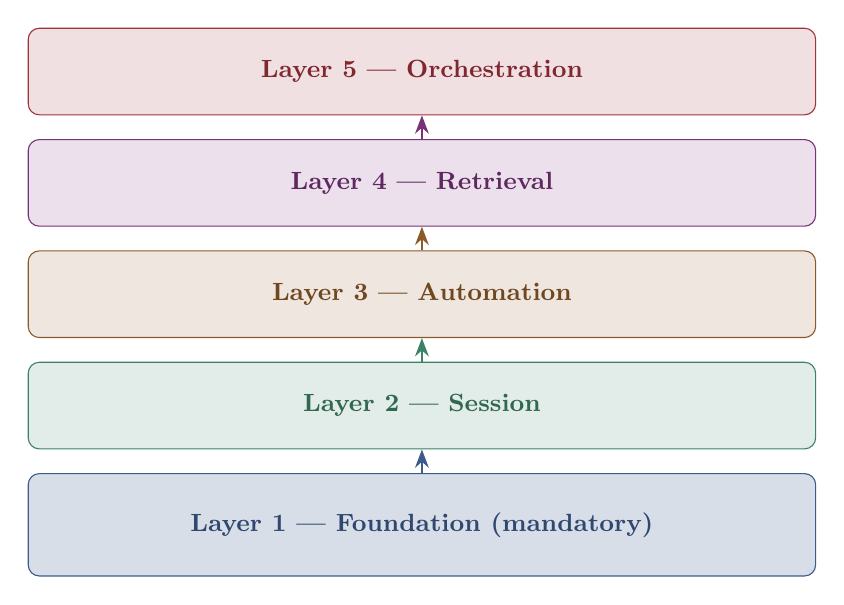
\begin{tikzpicture}[
  box/.style={rectangle, rounded corners=4pt, minimum width=10cm,
              minimum height=1.1cm, text centered, font=\small\bfseries,
              inner sep=8pt},
  arrow/.style={->, >=Stealth, thick}
]

\node[box, fill=l5color!15, draw=l5color, text=l5color!80!black]
  (l5) {Layer 5 --- Orchestration};
\node[box, fill=l4color!15, draw=l4color, text=l4color!80!black, below=0.3cm of l5]
  (l4) {Layer 4 --- Retrieval};
\node[box, fill=l3color!15, draw=l3color, text=l3color!80!black, below=0.3cm of l4]
  (l3) {Layer 3 --- Automation};
\node[box, fill=l2color!15, draw=l2color, text=l2color!80!black, below=0.3cm of l3]
  (l2) {Layer 2 --- Session};
\node[box, fill=l1color!20, draw=l1color, text=l1color!80!black, below=0.3cm of l2, 
      minimum height=1.3cm]
  (l1) {Layer 1 --- Foundation (mandatory)};

\draw[arrow, color=l1color] (l1.north) -- (l2.south);
\draw[arrow, color=l2color] (l2.north) -- (l3.south);
\draw[arrow, color=l3color] (l3.north) -- (l4.south);
\draw[arrow, color=l4color] (l4.north) -- (l5.south);

\end{tikzpicture}
\end{center}

\subsection{What Each Layer Owns}

\begin{center}
\begin{tabular}{@{}p{3.5cm}p{2cm}p{7cm}@{}}
\toprule
\textbf{Responsibility} & \textbf{Layer} & \textbf{Mechanism} \\
\midrule
Permanent storage & 1 & Plain text files in folder hierarchy \\
Metadata & 1 & YAML frontmatter inside each file \\
Version history & 1 & Versioned triplet files (v01, v02\ldots) \\
Project narrative & 1 & THREAD.md checkpoint log \\
Library navigation & 1 & MAP.md traversal index \\
Session control & 1 & Master prompt + commands \\
Context resume & 1 & instructions.md pasted into new sessions \\
\midrule
Persona auto-loading & 2 & Platform workspace system prompt \\
Session preference memory & 2 & Platform memory feature \\
Reduced startup friction & 2 & Project workspace pre-loaded context \\
\midrule
File saving automation & 3 & checkpoint.py parses and saves \\
THREAD.md automation & 3 & checkpoint.py appends log entry \\
MAP.md automation & 3 & update-map.py \\
\midrule
Semantic search & 4 & Embedding model + vector store \\
Automatic context loading & 4 & search.py + load-context.py \\
Filtered retrieval & 4 & Frontmatter metadata + vector similarity \\
\midrule
Folder navigation by AI & 5 & MCP client reads library directly \\
Scheduled tasks & 5 & cron + API scripts \\
Cross-project synthesis & 5 & Synthesis agent reads all THREAD.md \\
Pipeline automation & 5 & run-pipeline.py orchestrates agents \\
Team collaboration & 5 & Shared folder + merge protocol \\
\bottomrule
\end{tabular}
\end{center}

\subsection{Implementation Sequence}

The recommended implementation sequence is strictly bottom-up.
Do not skip layers.

\begin{enumerate}
  \item \textbf{Layer 1:} Create the folder structure. Move existing
        files into \texttt{inbox/}. Sort one project. Create its
        \texttt{THREAD.md} and \texttt{persona.md}. Save
        \texttt{MASTER-PROMPT.md} to the library root. Run one
        complete session using the master prompt. Call one checkpoint
        manually. This is the proof of concept.

  \item \textbf{Layer 2:} Create a Claude Project for the first
        active project. Load the persona and structural conventions
        into the system prompt. Run three sessions from the project
        workspace. Verify that sessions start faster and the AI
        behaves consistently.

  \item \textbf{Layer 3:} Write the checkpoint script. Test it on
        a real checkpoint output. Verify that all four files are
        saved correctly and \texttt{THREAD.md} and \texttt{MAP.md}
        are updated accurately. Use it for ten real checkpoints
        before adding Layer 4.

  \item \textbf{Layer 4:} Choose an embedding model and vector store.
        Index the library. Run ten retrieval queries across different
        topics. Verify that results are accurate and relevant. Integrate
        retrieval into the session start workflow for one month.

  \item \textbf{Layer 5:} Implement MCP connection first, before any
        scheduling or pipelines. Run ten sessions via the MCP client.
        Then implement one scheduled task (the weekly synthesis is
        recommended as the first). Verify it produces useful output
        for one month before implementing pipelines.
\end{enumerate}

\subsection{Time Estimates}

\begin{center}
\begin{tabular}{@{}lll@{}}
\toprule
\textbf{Layer} & \textbf{Setup time} & \textbf{Time to stable use} \\
\midrule
1 & 30--60 minutes & 2--3 active projects \\
2 & 15--30 minutes per project & Immediate after setup \\
3 & 2--4 hours (scripting) & After 10 real checkpoints \\
4 & 4--8 hours (setup + indexing) & After 1 month of retrieval use \\
5 & 8--20 hours (MCP + scheduling) & After 3 months of Layer 4 use \\
\bottomrule
\end{tabular}
\end{center}

% ---------------------------------------------------------------
\section{Document Index}

The following documents make up the complete Layer 1 reference set.
All should be stored in the root of \texttt{AI-Library/}.

\begin{center}
\begin{tabular}{@{}lp{9cm}@{}}
\toprule
\textbf{File} & \textbf{Contents} \\
\midrule
\texttt{MASTER-PROMPT.md} &
The system prompt pasted at the start of every AI session.
Contains the complete Layer 1 operating instructions for any AI model. \\
\texttt{MASTER-PROMPT.tex} &
LaTeX source for the master prompt document. Includes component
reference, usage instructions, and the raw prompt in a verbatim block. \\
\texttt{USER-GUIDE.tex} &
Complete Layer 1 user guide. Philosophy, all file conventions,
project structure, checkpoint ritual, MAP.md, and troubleshooting. \\
\texttt{ARCHITECTURE.tex} &
This document. Complete five-layer architecture reference. \\
\bottomrule
\end{tabular}
\end{center}

% ---------------------------------------------------------------
\section*{Colophon}

\vspace{8pt}
\hrule height 0.4pt
\vspace{12pt}

\begin{center}
{\small\texttt{AI-Library / ARCHITECTURE.tex} \quad Version 1.0 \quad \today}\\[6pt]
{\small Plain text. Open format. No vendor. No application required. No expiry.}\\[4pt]
{\footnotesize
Layer 1 is the only mandatory layer.\\
Every additional layer adds convenience.\\
None of them changes where the truth lives.
}
\end{center}

\end{document}
